
% % \noindent \textbf{Academic Employment}

% % \noindent Post doctor in Macro and Green Finance Lab, School of National Development, Beijing University.

% % ~\\

% % \noindent \textbf{Education}]




% Vita.te

\subsubsection*{ACADEMIC EMPLOYMENT}
\textbf{Post doctor} \hfill \textbf{2024--} \\
Peking University, School of National Development \hfill \textit{Beijing, China}
\\[8pt]


\subsubsection*{EDUCATION}
\textbf{Doctor of Philosophy in Public Administration} \hfill \textbf{2019--2024} \\
Pennsylvania State University \hfill \textit{Pennsylvania, America}
\\[12pt]
\noindent \textbf{Master of Science in Applied Economics} \hfill \textbf{2017--2019} \\
The Johns Hopkins University \hfill \textit{Washington DC, America}
\\[12pt]
\noindent \textbf{Bachelor in Economics} \hfill \textbf{2012--2016} \\
Central University of Finance and Economics \hfill \textit{Beijing, China}
\\[8pt]


\subsubsection*{RESEARCH EXPERIENCE}
\noindent \textbf{Graduate Research Assistant} \hfill \textbf{2019--2021} \\
Pennsylvania State University \hfill \textit{Pennsylvania, America}\\
Professor: Ran Bing, Odd Stalebrink
\\[12pt]
\noindent \textbf{Research Assistant} \hfill \textbf{2019} \\
The Johns Hopkins University \hfill \textit{Washington DC, America}\\
Professor: Sang-Sub Lee
\\[12pt]
\noindent \textbf{Research Assistant} \hfill \textbf{2019--2021} \\
Central University of Finance and Economics \hfill \textit{Beijing, China}\\
Professor: Bai Yanfeng
\\[8pt]

\subsubsection*{TEACHING EXPERIENCE}
\textbf{Adjunct Professor} \hfill \textbf{2022} \\
Pennsylvania State University \hfill \textit{Pennsylvania, America}\\
Course: International Politics
\\[12pt]
\noindent \textbf{Adjunct Professor} \hfill \textbf{2022} \\
Pennsylvania State University \hfill \textit{Pennsylvania, America}\\
Course: Comparative Politics
\\[12pt]
\noindent \textbf{Teaching Assistant} \hfill \textbf{2017--2018} \\
The Johns Hopkins University \hfill \textit{Washington DC, America}\\
Course: Econometrics \\
Professor: Lixiong Li
\\[12pt]
\noindent \textbf{Teaching Assistant} \hfill \textbf{2018} \\
Purdue University \hfill \textit{Beijing, China}\\
Course: Financial Accounting \\
Professor: Frank Kane
\\[12pt]
\noindent \textbf{Teaching Assistant} \hfill \textbf{2018} \\
Purdue University \hfill \textit{Beijing, China}\\
Course: Financial Accounting \\
Professor: Frank Kane
\\[8pt]

\subsubsection*{ACADEMIC CONFERENCE AND PRESENTATION PROCEEDINGS}
\noindent \textbf{American Society for Public Administration Conference} \hfill \textbf{Nov 2019} \\
Presenter \hfill \textit{Washington D.C, America}\\
Title: Political Party Control and Intergovernmental Transfer under Fiscal Federalism—a Longitudinal Study
\\[12pt]
\noindent \textbf{Northeast Conference on Public Administration Conference} \hfill \textbf{Mar 2020} \\
Presenter \hfill \textit{New York, America}\\
Title: Political Party Control and Intergovernmental Transfer under Fiscal Federalism—a Longitudinal Study
\\[12pt]
\noindent \textbf{American Society for Public Administration Conference} \hfill \textbf{Nov 2021} \\
Presenter \hfill \textit{San Diego, America}\\
Title: Fiscal Behavior of Central and Local Governments under Asymmetric Setting—a Game Theory Model Setting
\\[12pt]
\noindent \textbf{American Society for Public Administration Conference} \hfill \textbf{Oct 2021} \\
Presenter \hfill \textit{Online, America}\\
Title: Grants in Aid on Subnational Tax Collection Behavior: an Panel Data Empirical Evidence
\\[8pt]
% 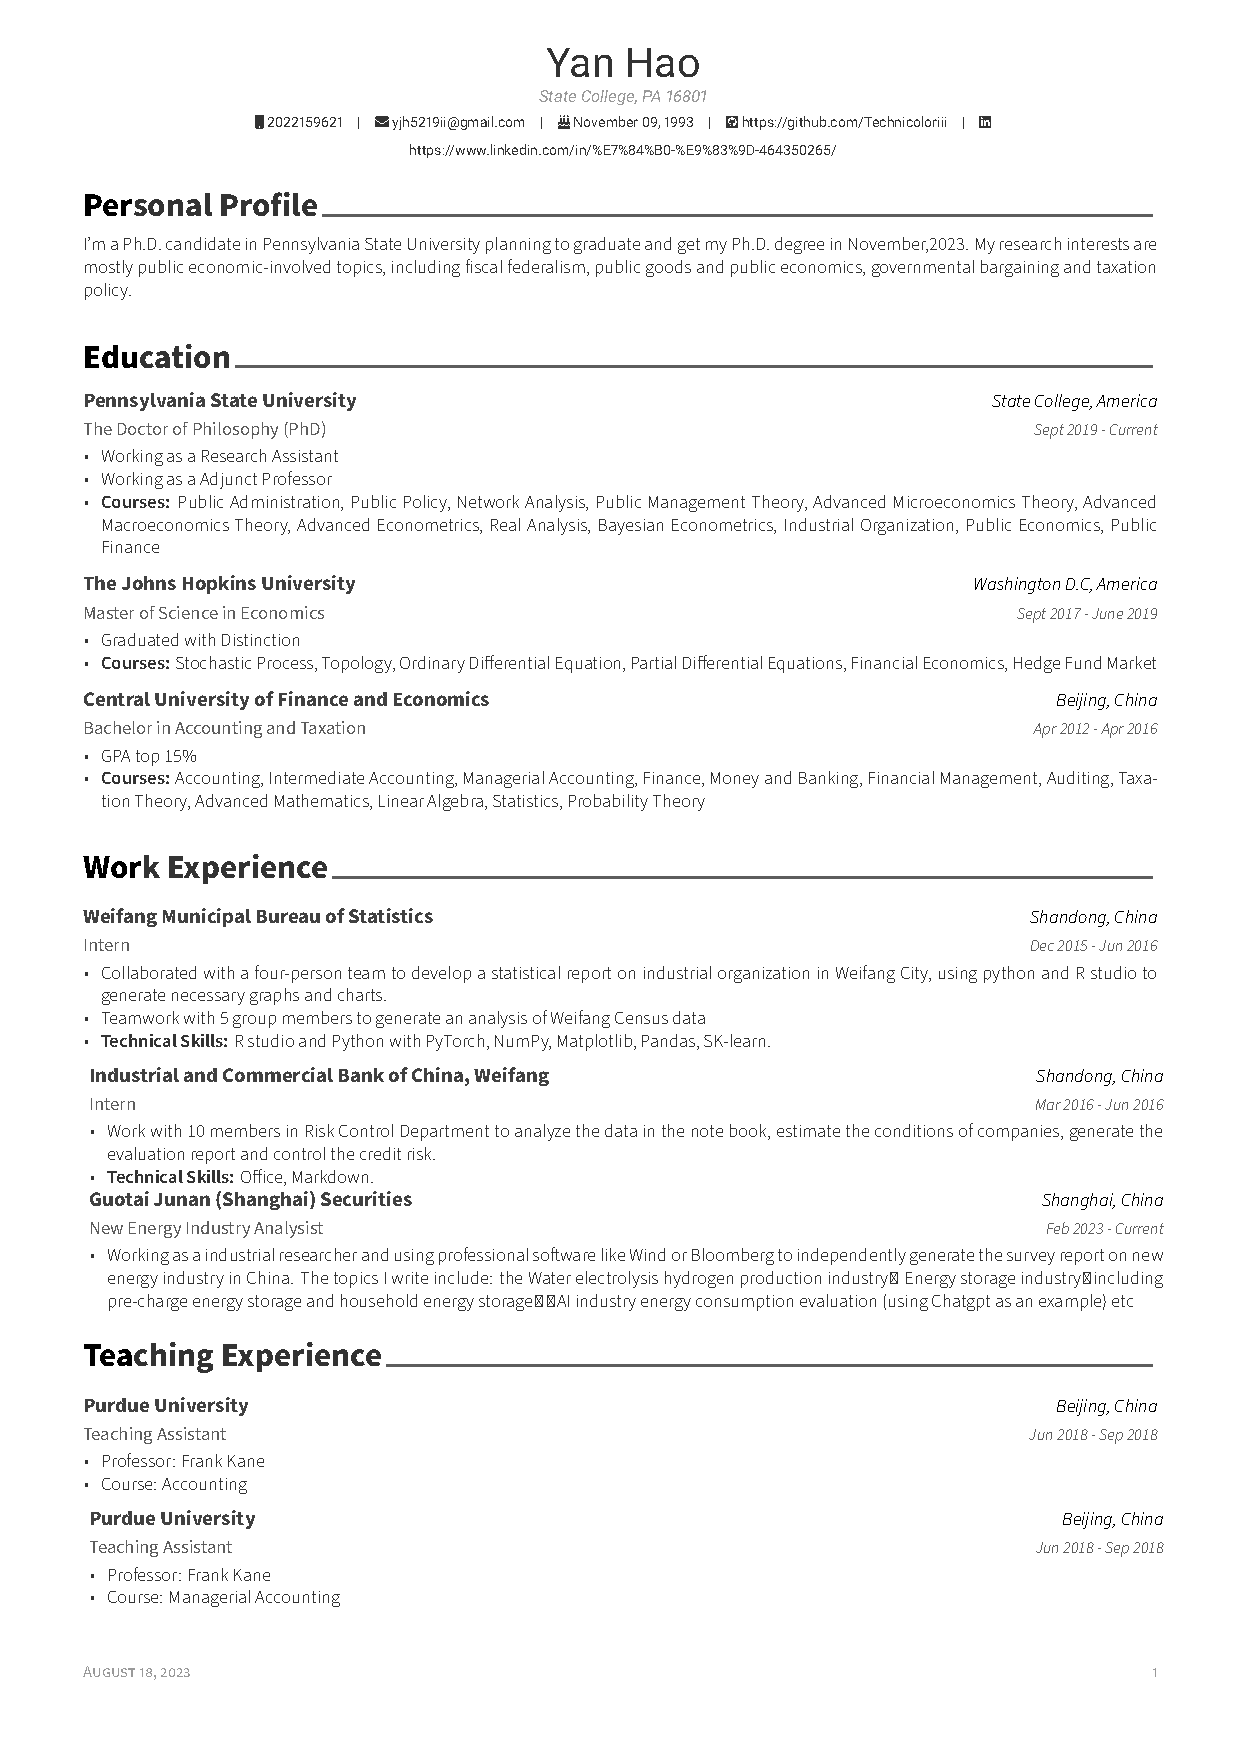
\includepdf{Resume_Yan_Hao_English_Version.pdf}

\subsubsection*{PAPERS}
\noindent \textbf{Working Paper:} Yan Hao, \textit{Intergovernmental Transfer Decision---an Outcome of the Interaction between Central and Local Government}
\\[12pt]
\noindent \textbf{Working Paper:} Odd Stalebrink, Yan Hao, \textit{Political Party Control and Intergovernmental Grants: a Panel Data Analysis}
\\[12pt]
\noindent \textbf{Working Paper:} Yan Hao, \textit{Effect of Grants Restriction on Subnational Governments' Revenue Collection Effort--a Kalman Filter Application}

